%
% Barren Planet - User Manual
% Main document source
%
% Copyright (C) Damian Gareth Walker 2022
% Manual Sections: Winning the Battle
%
% Structure:
% Victory Conditions
% - Victory Points
% - Complete Destruction
% Debriefing
% The Next Battle
%

% Chapter Title
\chapter{Winning the Battle}

% Victory Conditions
\noindent
There are two ways to win a battle. One is to occupy all of the {\it Victory Points} on the map. The other is complete annihilation of the enemy forces.

% Victory Points
{\it Victory Points} are positions on the map that must be occupied to secure victory. They are indicated by small circles in the top left of their squares. A red circle is an unoccupied victory point. Victory points occupied by Nuvutech turn white, while those occupied by Avuscorp turn blue.

% An image showing victory points
\begin{figure}[h]
  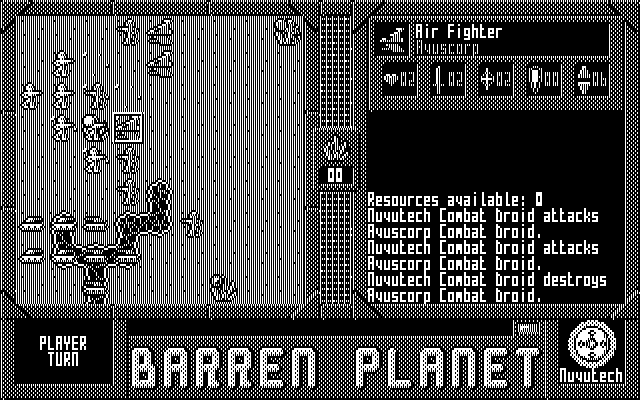
\includegraphics[width=\textwidth]{victory-points}
  \caption{Three victory points are visible on the map. The one on the left is occupied by Nuvutech. The upper right one is occupied by Avuscorp. The lower right one is unnocupied.}
\end{figure}

% Winning by Occupation
If there are such victory points on the map, and if you occupy them all, then you instantly win the battle. You do not need to destroy all the enemy units; seizing all of the important victory points is enough to secure victory.

% Complete Annihilation
If there are no victory points on the map, or if your forces are too few to occupy them all, then the only other way to win the battle is complete annihilation of the enemy. You could also do this for fun, and ignore the victory points even if you have enough units to occupy them. But such a war of attrition will take much longer than occupying the victory positions so it is best avoided if possible.

% The Debriefing
\section{The Mission Debriefing}

% Victory
\noindent
If you win a battle, you will be taken straight to the {\it Mission Debriefing} screen. The text in the top right window will describe how you did, and what effect your victory will have upon the campaign. The map in the top left window shows the final battle positions.

% The Mission Debriefing image
\begin{figure}[h]
  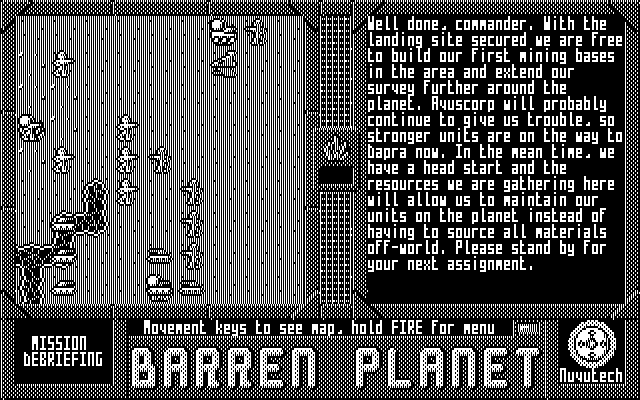
\includegraphics[width=\textwidth]{mission-debriefing}
  \caption{The Mission Debriefing: Nuvutech has won the battle by
    occupying all the victory points.}
\end{figure}

% Controls
The Mission Debriefing works much like the briefing: you can scroll around the map with the movement controls to reveal the full battlefield. The {\it fire} control, as always, brings up the menu.

% Acknowledgement
To acknowledge the debriefing and continue the campaign, tap {\it fire} which brings up the menu and chooses the default option {\it Acknowledge}. You will then proceed to the next battle or, if you have won the campaign, to the {\it New Game} screen.

% Loss
If you have lost the battle, which would usually occur in your opponent's turn, then you will first be taken to the {\it Turn Report} screen so that you can see what happened. Once you have watched the report, then you will see the Mission Debriefing as described already.

% The Next Battle
\section{The Next Battle}

% Introductory
\noindent
A campaign is a series of interlinked battles. It isn't a fixed linear sequence, though. The outcome of each battle will determine which battle is fought next. This means that both sides have a chance to influence events on the strategic level, and the game becomes interesting for both players. It also means that you might encounter different battles in each play through of the campaign.

% Structure of First Landing
In the {\it First Landing} campaign, winning a battle is likely to take the victorious player to a scenario where their capabilities are increased. For instance, the winner of the first battle will proceed to a mission in which they have established a mining base and are able to start repairing their units. Winning later battles may introduce new units to the victor, or the ability to build units at will.

% The first appearance of the Mining Base
\begin{figure}[h]
  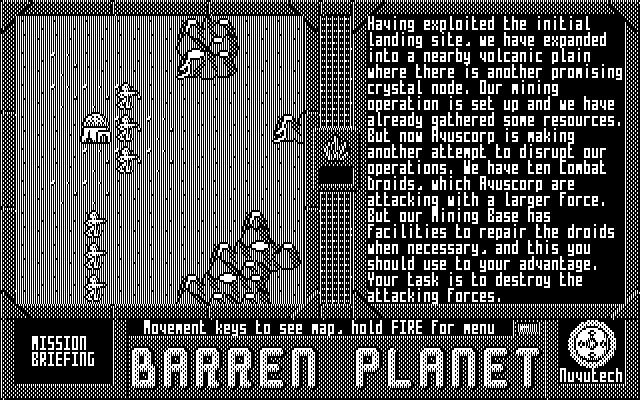
\includegraphics[width=\textwidth]{second-scenario}
  \caption{In the next battle, the victorious player finally
    establishes a Mining Base.}
\end{figure}

% Final Victory
As the campaign draws to its close, battles will be encountered where victory for one player will give them victory for the entire campaign. Once a player wins such a battle, the debriefing will award outright victory and the game will end. But it will take many battles before this happens.
